\documentclass[xcolor={dvipsnames}]{beamer}
%\usepackage[utf8]{inputenc}
\usetheme{CambridgeUS}

%-------------------------------------------------------------------------------
%          -Packages nécessaires pour écrire en Français et en UTF8-
%-------------------------------------------------------------------------------
\usepackage[utf8]{inputenc}
\usepackage[frenchb]{babel}
\usepackage[T1]{fontenc}
\usepackage{lmodern}
\usepackage{textcomp}

%-------------------------------------------------------------------------------

%-------------------------------------------------------------------------------
%                          -Outils de mise en forme-
%-------------------------------------------------------------------------------
\usepackage{hyperref}
\hypersetup{pdfstartview=XYZ}
\usepackage{enumerate}
\usepackage{graphicx}
%\usepackage{multicol}
%\usepackage{tabularx}

%\usepackage{anysize} %%pour pouvoir mettre les marges qu'on veut
%\marginsize{2.5cm}{2.5cm}{2.5cm}{2.5cm}

\usepackage{indentfirst} %%pour que les premier paragraphes soient aussi indentés
\usepackage{verbatim}
%\usepackage[table]{xcolor}  
%\usepackage{multirow}
\usepackage{ulem}
%-------------------------------------------------------------------------------


%-------------------------------------------------------------------------------
%                  -Nécessaires pour écrire des mathématiques-
%-------------------------------------------------------------------------------
\usepackage{amsfonts}
\usepackage{amssymb}
\usepackage{amsmath}
\usepackage{amsthm}
\usepackage{tikz}
\usepackage{xlop}
\usepackage[output-decimal-marker={,}]{siunitx}
%-------------------------------------------------------------------------------


%-------------------------------------------------------------------------------
%                    - Mise en forme 
%-------------------------------------------------------------------------------

\newcommand{\bu}[1]{\underline{\textbf{#1}}}


\usepackage{ifthen}


\newcommand{\ifTrue}[2]{\ifthenelse{\equal{#1}{true}}{#2}{$\qquad \qquad$}}

\newcommand{\kword}[1]{\textcolor{red}{\underline{#1}}}


%-------------------------------------------------------------------------------



%-------------------------------------------------------------------------------
%                    - Racourcis d'écriture -
%-------------------------------------------------------------------------------

% Angles orientés (couples de vecteurs)
\newcommand{\aopp}[2]{(\vec{#1}, \vec{#2})} %Les deuc vecteurs sont positifs
\newcommand{\aopn}[2]{(\vec{#1}, -\vec{#2})} %Le second vecteur est négatif
\newcommand{\aonp}[2]{(-\vec{#1}, \vec{#2})} %Le premier vecteur est négatif
\newcommand{\aonn}[2]{(-\vec{#1}, -\vec{#2})} %Les deux vecteurs sont négatifs

%Ensembles mathématiques
\newcommand{\naturels}{\mathbb{N}} %Nombres naturels
\newcommand{\relatifs}{\mathbb{Z}} %Nombres relatifs
\newcommand{\rationnels}{\mathbb{Q}} %Nombres rationnels
\newcommand{\reels}{\mathbb{R}} %Nombres réels
\newcommand{\complexes}{\mathbb{C}} %Nombres complexes


%Intégration des parenthèses aux cosinus
\newcommand{\cosP}[1]{\cos\left(#1\right)}
\newcommand{\sinP}[1]{\sin\left(#1\right)}

%Fractions
\newcommand{\myfrac}[2]{{\LARGE $\frac{#1}{#2}$}}

%Vocabulaire courrant
\newcommand{\cad}{c'est-à-dire}

%Droites
\newcommand{\dte}[1]{droite $(#1)$}
\newcommand{\fig}[1]{figure $#1$}
\newcommand{\sym}{symétrique}
\newcommand{\syms}{symétriques}
\newcommand{\asym}{axe de symétrie}
\newcommand{\asyms}{axes de symétrie}
\newcommand{\seg}[1]{$[#1]$}
\newcommand{\monAngle}[1]{$\widehat{#1}$}
\newcommand{\bissec}{bissectrice}
\newcommand{\mediat}{médiatrice}
\newcommand{\ddte}[1]{$[#1)$}

%Figures
\newcommand{\para}{parallélogramme}
\newcommand{\paras}{parallélogrammes}
\newcommand{\myquad}{quadrilatère}
\newcommand{\myquads}{quadrilatères}
\newcommand{\co}{côtés opposés}
\newcommand{\diag}{diagonale}
\newcommand{\diags}{diagonales}
\newcommand{\supp}{supplémentaires}
\newcommand{\car}{carré}
\newcommand{\cars}{carrés}
\newcommand{\rect}{rectangle}
\newcommand{\rects}{rectangles}
\newcommand{\los}{losange}
\newcommand{\loss}{losanges}


%----------------------------------------------------


\usepackage{../../../../pas-math}
\usepackage{../../../../moncours_beamer}


\graphicspath{{../img/}}

\title{Exponentielles et logarithme décimal}
\author{}\institute{}


\AtBeginSection[]
{
	\begin{frame}
		\frametitle{Sommaire}
		\tableofcontents[currentsection, hideallsubsections]
	\end{frame} 
}


\AtBeginSubsection[]
{
	\begin{frame}
		\frametitle{Sommaire}
		\tableofcontents[currentsection, currentsubsection]
	\end{frame} 
}

\begin{document}



\begin{frame}
  \titlepage 
\end{frame}

\section{Fonction exponentielle de base $q$}

\subsection{Définition}



\begin{frame}
\begin{mydef}
	$q$ est un nombre strictement positif ($q > 0$).
	La fonction qui à tout nombre $x$ associe $q^x$, est appelée \kw{fonction exponentielle} de base $q$.
\end{mydef}\pause

\begin{myex}
	\begin{itemize}
		\item La fonction $f$, définie par $f(x)=2^x$, est la \kw{fonction exponentielle de base $2$}. 
		\item La fonction $g$, définie par $g(x)=0,5^x$, est la \kw{fonction exponentielle de base $0,5$}.
	\end{itemize}
	
\end{myex}

\end{frame}

\subsection{Valeurs particulières et variations}
\begin{frame}
\begin{myprops}
	\begin{enumerate}
		\item Valeurs particulières :
		
		\begin{center}
			\begin{align*}
			q^0 = 1 \qquad\qquad\qquad\qquad q^1 = q 			
			\end{align*}
		\end{center}
		
		
		\item Variations :
		\begin{itemize}
			\item Si \kw{$q > 0$}, alors la fonction est \kw{croissante}.
			\item Si \kw{$q < 0$}, alors la fonction est \kw{décroissante}.
		\end{itemize}
	\end{enumerate}
\end{myprops}
\end{frame}
%\begin{columns}[c]
%	\begin{column}{6cm}
%		\begin{itemize}
%			\item $f(x)=2x$
%			\item $g(x)=-x+2$
%		\end{itemize}
%	\end{column}
%	\begin{column}{6cm}
%		\begin{itemize}
%			\item $h(x)=3x-4$
%			\item $i(x)=5$
%		\end{itemize}
%	\end{column}				
%\end{columns}

\begin{frame}
\begin{myex}
	\begin{columns}{}
		\begin{column}{6cm}
					
			$f(x)= 2^x$, $2 > 1$\\
			la fonction $f$ est croissante
		
			\begin{center}
				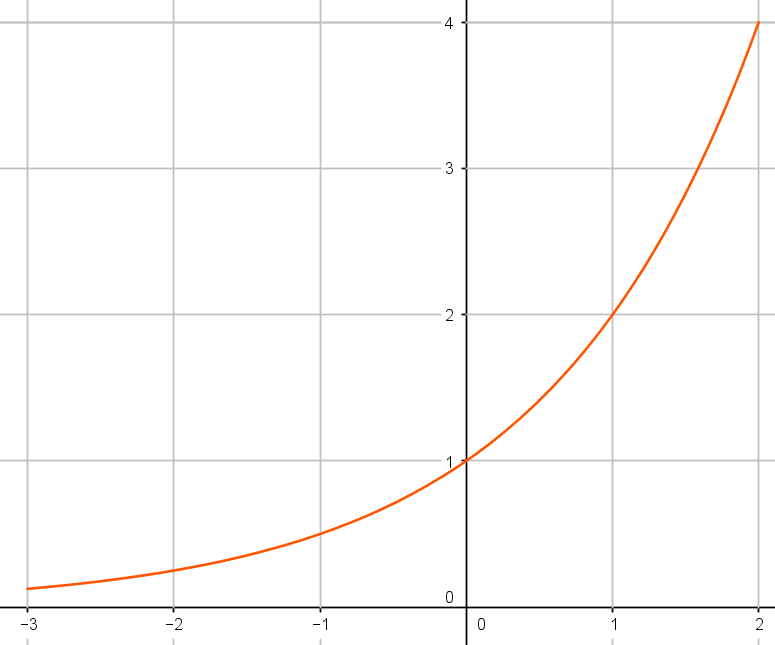
\includegraphics[scale=0.25]{var1}
			\end{center}
		
		\end{column}
		
		\begin{column}{6cm}
			$g(x)= 0,5^x$, $0,5 > 1$\\
			la fonction $g$ est décroissante
			
			\begin{center}
				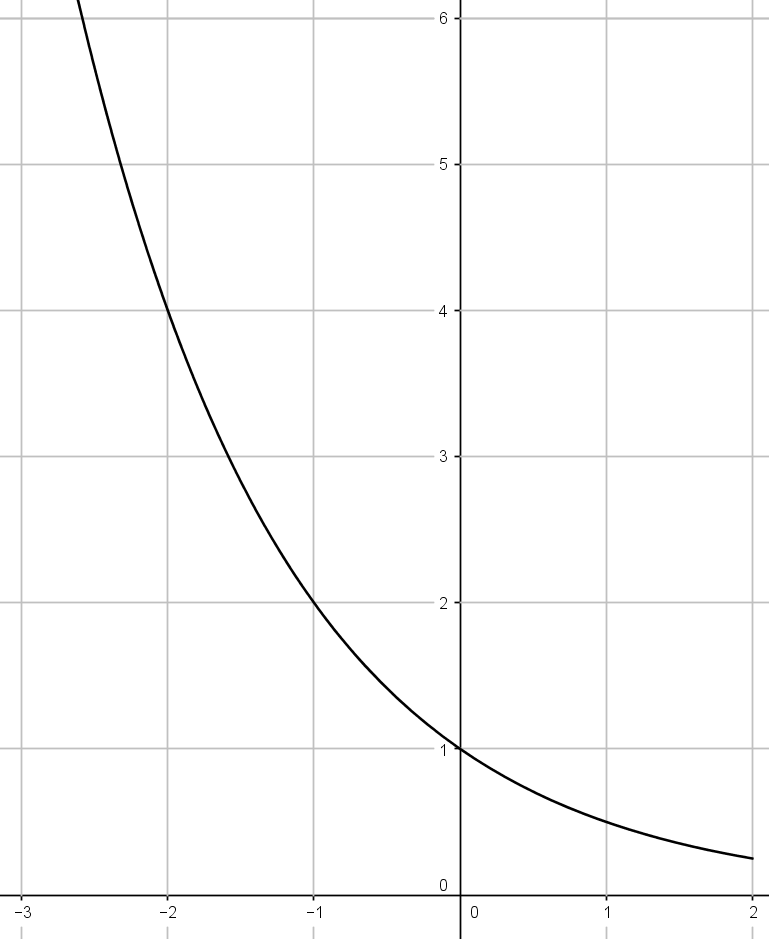
\includegraphics[scale=0.2]{var2}
			\end{center}
			
		\end{column}
		
	\end{columns}
\end{myex}

\end{frame}

\subsection{Règles de calcul}

\begin{frame}
	\begin{myprops}
		Les règles de calculs sont les mêmes que pour les puissances entières.\\
		$a$ et $b$ sont deux nombres quelconques et $q$ un nombre strictement positif.
		
		\begin{align*}
		q^a = q^b &\Leftrightarrow a = b\\
		q^x \times q^y &= q^{a+b}\\
		\frac{q^a}{q^b} &= q^{a-b}\\
		(q^a)^b &= q^{a \times b}
		\end{align*}
		\end{myprops}
			
\end{frame}

\begin{frame}
	\begin{myex}
		
		\begin{align*}
		2^{-4} \times 2^{1,5} &= 2^{-2,5}\\\\
		\frac{0,1^3}{0,1^{1,8}} &= 0,1^{1,2}\\\\
		(3^{0,4})^{-2} &= 3^{-0,8}
		\end{align*}
	\end{myex}
\end{frame}


\section{Fonction logarithme décimal}

\subsection{Définition}

\begin{frame}
	\begin{mydef}
		$a$ est un nombre strictement positif ($a>0$), le nombre $b$ tel que \kw{$10^b=a$}, est le \kw{logarithme décimal} de a, noté $\log a$.
	\end{mydef}
\end{frame}


\subsection{Valeurs particulières et variations}

\begin{frame}
	\begin{myprops}
		\begin{enumerate}
			\item Valeurs particulières :
			\begin{align*}
			\log 1 &= 0 \\
			\log 10 &= 1\\
			\log 100 &= 2
			\end{align*}
			
			\item Signe et variations :
			\begin{itemize}
				\item La fonction $\log x$ est \kw{croissante} pour $x > 0$.
				\item Si $0 \leq x < 1$, alors $\log x$ est négatif.
				\item Si $x \geq 1$, alors $\log x$ est positif.
			\end{itemize}			
			
			\begin{center}
				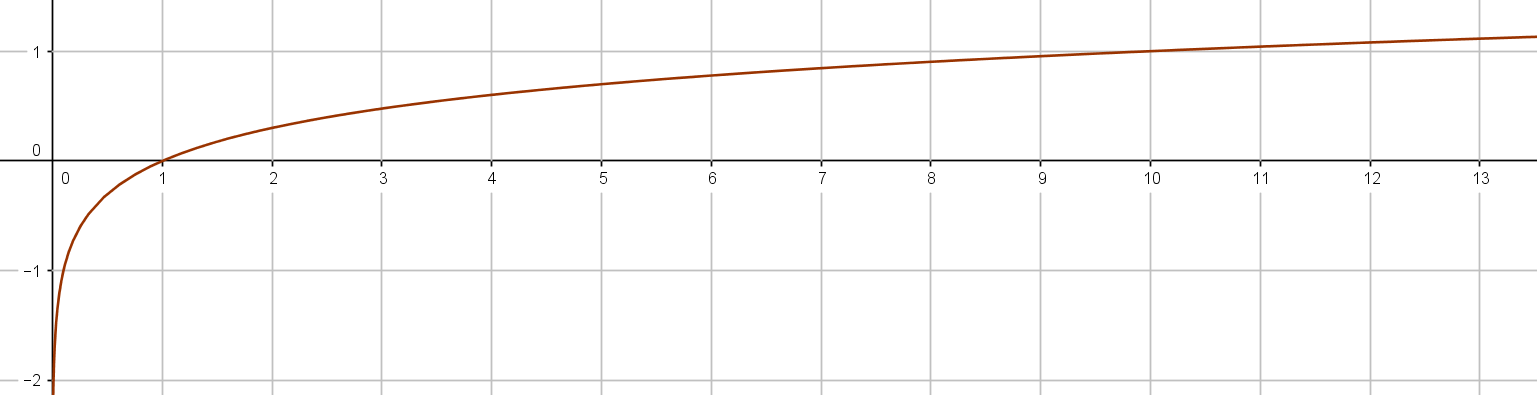
\includegraphics[scale = 0.22]{var_log}
			\end{center}	
		\end{enumerate}
		
		
	\end{myprops}
\end{frame}


\subsection{Règles de calcul}
\begin{frame}
	\begin{myprops}
		$a$ et $b$ sont deux nombres strictement positifs :
		
		\begin{align*}
		\log a = b &\Leftrightarrow a = 10^b \\
		10^b = a &\Leftrightarrow b = \log a \\
		\log a = \log b &\Leftrightarrow a = b \\
		\log a < \log b &\Leftrightarrow a < b \\
		\log (a \times b) &= \log a + \log b \\
		\log  \left( \frac{a}{b} \right) &= \log a - \log b \\
		\log(a^x) &= x \times \log a 
		\end{align*}
	\end{myprops}	
\end{frame}

\end{document}